% Lecture Template for ME3023 -  Measurements in Mechanical Systems - Tennessee Technological University
% Spring 2020 - Summer 2020 - Fall 2020 - Spring 2021 - Summer 2021
% Tristan Hill, May 07, 2020 - June 12, 2020 - July 08, 2020 - Novemeber 02, 2020 - March 28, 2021 - May 25, 2021 - August 21, 2022

% Fall 2023 - condensing and streamlining lectures by combining topics into a single PDF under the module name
%			  this will simplify file and link management as well as make lectures easier to use in class
%			- added image/ to clean directory and reduce redundancy, specific to module for now  

% Module Name: - Introduction
% Topic 1 - General Measurement System
% Topic 2 - Types of Variables 
% Topic 3 - Experimental Test Plan  ! needs improvement ! 

\documentclass[fleqn]{beamer} % for presentation (has nav buttons at bottom)

\usepackage{/home/thill/courses/measurements/lectures/measurements_lectures}
%\usepackage{/mnt/c/Users/thill/Documents/courses/measurements/lectures/measurements_lectures}

\author{ME3023 - Measurements in Mechanical Systems} % original formatting from Mike Renfro, September 21, 2004

\newcommand{\MNUM}{1\hspace{2mm}} % module number 
\newcommand{\moduletitle}{Introduction}
%\newcommand{\topictitle}{General Measurement System} 

\newcommand{\sectionItitle}{General Measurement System}
\newcommand{\sectionIItitle}{Types of Variables}
\newcommand{\sectionIIItitle}{Experimental Test Plan}
\newcommand{\sectionIVtitle}{Numbers and Storage}

\newcommand{\sectionIsubsectionItitle}{Definition of a Measurement}
\newcommand{\sectionIsubsectionIItitle}{Measurement System Stages}
\newcommand{\sectionIsubsectionIIItitle}{Brainstorming Activity}
\newcommand{\sectionIsubsectionIVtitle}{Examples in Mechcanical Engineering}

\newcommand{\sectionIIsubsectionItitle}{Measured Variable}
\newcommand{\sectionIIsubsectionIItitle}{Independent and Dependent Variables}
\newcommand{\sectionIIsubsectionIIItitle}{Controlled Variables and Parameters}
\newcommand{\sectionIIsubsectionIVtitle}{Extraneous Variables}
\newcommand{\sectionIIsubsectionVtitle}{Class Activity: Measurement System Examples}

\newcommand{\sectionIIIsubsectionItitle}{Parameter Design Plan}
\newcommand{\sectionIIIsubsectionIItitle}{System and Tolerance Design Plan}
\newcommand{\sectionIIIsubsectionIIItitle}{Data Reduction Design Plan}
\newcommand{\sectionIIIsubsectionIVtitle}{Experimental Design Strategies}
\newcommand{\sectionIIIsubsectionVtitle}{Small Group Activity}

\newcommand{\sectionIVsubsectionItitle}{IV-I}
\newcommand{\sectionIVsubsectionIItitle}{IV-II}
\newcommand{\sectionIVsubsectionIIItitle}{IV-III}
\newcommand{\sectionIVsubsectionIVtitle}{IV-IV}
% custom box
\newsavebox{\mybox}

\title{Lecture Module - \moduletitle}

\date{Mechanical Engineering\vspc Tennessee Technological University}

\begin{document}

	\lstset{language=MATLAB,basicstyle=\ttfamily\small,showstringspaces=false}

	\frame{\titlepage \center\begin{framed}\Large \textbf{Topic \MNUM - \moduletitle}\end{framed} \vspace{5mm}}

	% Module Outline
	\begin{frame} 
		\large \textbf{Module \MNUM - \moduletitle} \vspace{3mm}\\

		\begin{itemize}
			\item Topic 1 - \hyperlink{sectionI}{\sectionItitle} \vspc % section I
			\item Topic 2 - \hyperlink{sectionII}{\sectionIItitle} \vspc % section II
			\item Topic 3 - \hyperlink{sectionIII}{\sectionIIItitle} \vspc % section III
			\item Topic 4 - \hyperlink{sectionIV}{\sectionIVtitle} \vspc % section IV
		\end{itemize}

	\end{frame}

	% section I
	\section{\sectionItitle}\label{sectionI}

		% section I Outline
		\begin{frame} 
			\large \textbf{Topic 1 - \sectionItitle} \vspace{3mm}\\

			\begin{itemize}
				\item \hyperlink{sectionIsubsectionI}{\sectionIsubsectionItitle} \vspc %  section I subsection I
				\item \hyperlink{sectionIsubsectionII}{\sectionIsubsectionIItitle} \vspc % section I subsection II
				\item \hyperlink{sectionIsubsectionIII}{\sectionIsubsectionIIItitle} \vspc % section I subsection III
				\item \hyperlink{sectionIsubsectionIV}{\sectionIsubsectionIVtitle} \vspc % section I subsection IV
			\end{itemize}
		\end{frame}
		
		% section I subsection I 
		\subsection{\sectionIsubsectionItitle}\label{sectionIsubsectionI}

			\begin{frame}
				\frametitle{\sectionIsubsectionItitle}

				\large{``A {\bf \BL measurement} is an act of assigning a specific value to a physical variable.''} \vspc
				{\tiny Text: Theory and Design of Mech. Meas.}

			\end{frame}

		% section I subsection II
		\subsection{\sectionIsubsectionIItitle}\label{sectionIsubsectionII}

			\begin{frame}
				\frametitle{\sectionIsubsectionIItitle}

				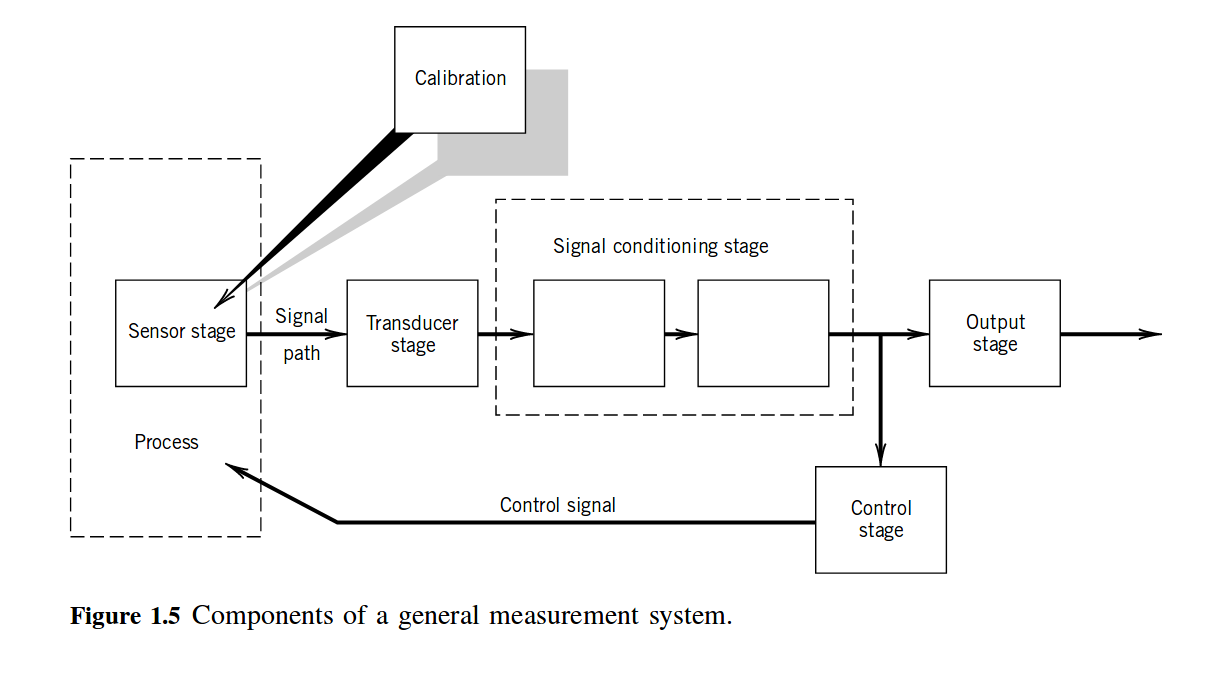
\includegraphics[scale=.325]{images/measurement_stages.png} \\
				{\tiny Image: Theory and Design of Mech. Meas.}
			\end{frame}

			\begin{frame}
				\frametitle{Sensor-Transducer Stage}
				a {\PR sensor}, a physical element that employs some natural phenomenon... ...to sense the variable being measured
				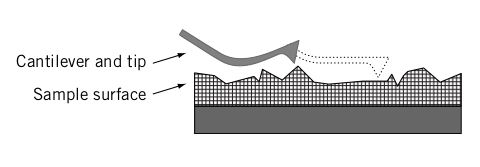
\includegraphics[scale=0.20]{images/sensor_stage.png}\hspace{5mm}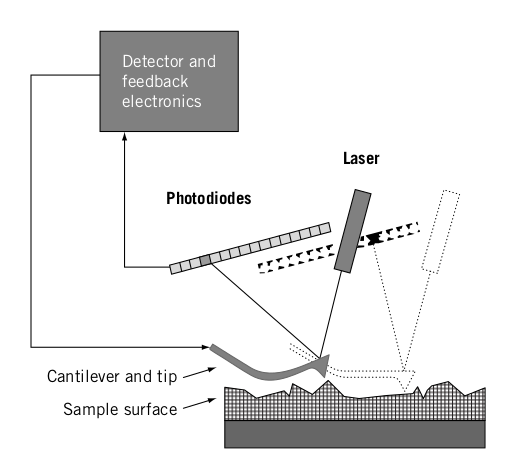
\includegraphics[scale=0.20]{images/sensor_transducer_stage.png}\\
               	{\footnotesize \hspace{10mm} {\PR Sensor} Stage \hspace{15mm} Sensor + {\GR Transducer} Stage} \vspace{3mm}

				A {\GR transducer} converts sensed information into a detectable signal \\
				{\tiny Text, Image: Theory and Design of Mech. Meas.}
			\end{frame}

			\begin{frame}
				\frametitle{Signal Conditioning Stage}

				\begin{multicols}{2}
				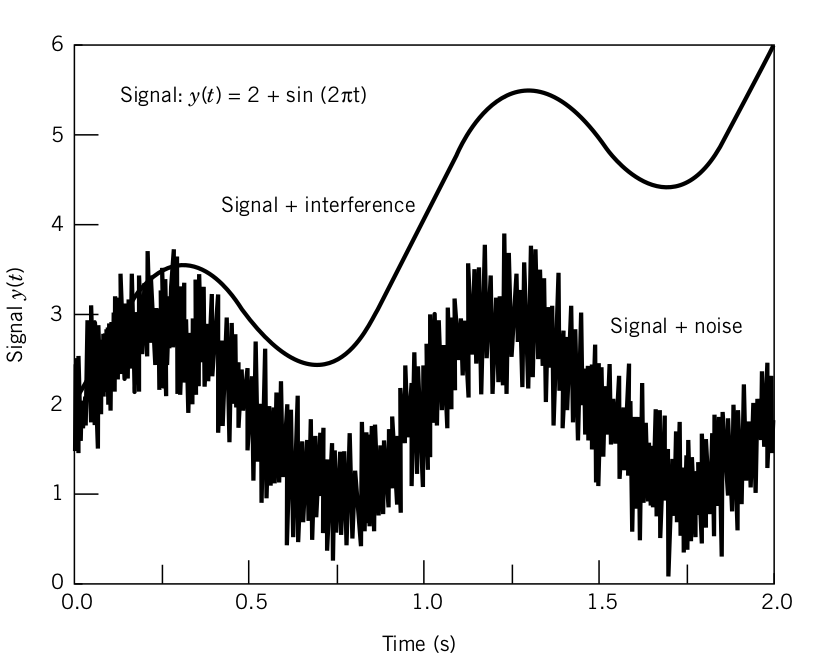
\includegraphics[scale=0.18]{images/signal_noise.png}

				\begin{itemize}
				\item Filtering
				\item Amplification
				\item Attenuation
				\item Excitation 
				\item Linearization
				\item Electrical Isolation
				\item Surge Protection
				\end{itemize}

				\end{multicols}

				Question: What is the the definition of {\BL signal}? \vspc

				{\tiny Image: Theory and Design of Mech. Meas.}
			\end{frame}

			\begin{frame}
				\frametitle{Defintion of a signal} {\footnotesize
				Signal (noun):
				{\it 4 a : an object used to transmit or convey information beyond the range of human voice 
				  	 b : the sound or image conveyed in telegraphy, telephony, radio, radar, or television 
				  	 c : a detectable physical quantity or impulse (such as a voltage, current, or magnetic field strength) by which messages or information can be transmitted } - \href{https://www.merriam-webster.com/dictionary/signal}{Merrian Webster} \vspace{3mm}

				{\it  	 In signal processing, a signal is a function that conveys information about a phenomenon.[1] Any quantity that can vary over space or time can be used as a signal to share messages between observers.[2] The IEEE Transactions on Signal Processing includes audio, video, speech, image, sonar, and radar as examples of signals.[3] A signal may also be defined as any observable change in a quantity over space or time (a time series), even if it does not carry information.} - \href{https://en.wikipedia.org/wiki/Signal}{Wikipedia}
				}  	 	
			\end{frame}

			\begin{frame}
				\frametitle{Output Stage}
				The {\BR output stage} indicates or records the value measured. This might be a simple readout
				display, a marked scale, or even a recording device such as a computer disk drive.

				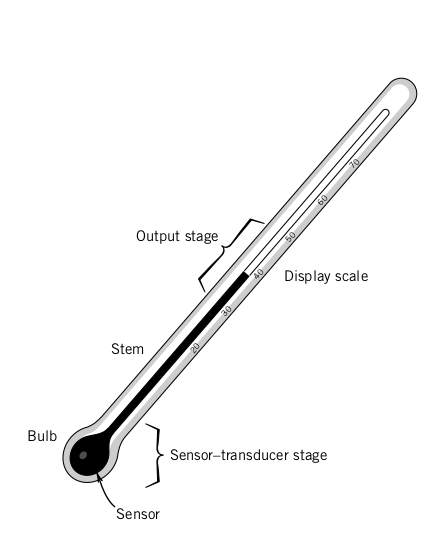
\includegraphics[scale=0.25]{images/bulb_thermometer.png} \hspace{10mm}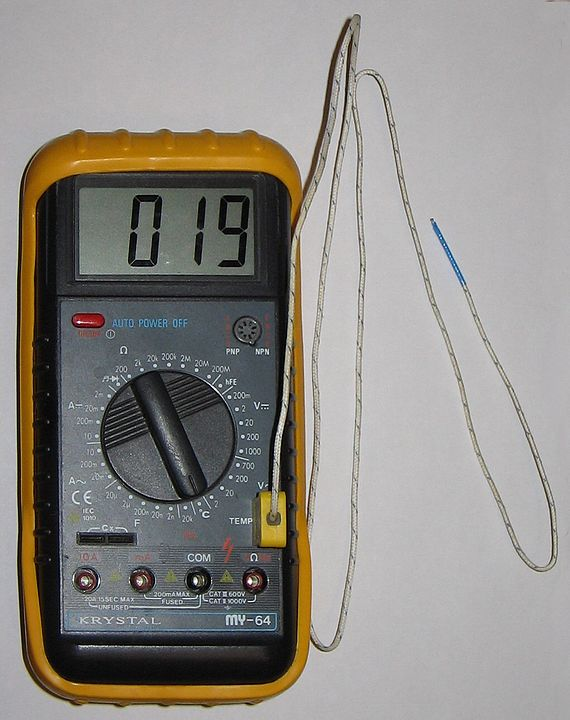
\includegraphics[scale=0.3]{images/thermocouple.jpg}

				{\tiny Image: Theory and Design of Mech. Meas. \hspace{20mm} Image: \href{https://en.wikipedia.org/wiki/Thermocouple}{Wikipedia} }
			\end{frame}

		% section I subsection III
		\subsection{\sectionIsubsectionIIItitle}\label{sectionIsubsectionIII}
			\begin{frame} 
				\frametitle{\sectionIsubsectionIIItitle}
				
				\begin{multicols}{2}
					\tiny

					{\bf Activity:} Team Brainstorm

					{\bf Duration:} $\sim 10$ minutes

					{\bf Groups:} 2-3 members

					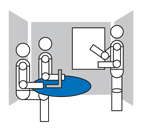
\includegraphics[scale=0.5]{images/Brainstorm_room.png}

					{\bf Topic:} Remote Probe Concept
					\begin{itemize}
						\item You are designing a remote probe to inspect an environment which can only be accessed from above. 
						\item The goal is to collect as much information as possible from the environment to prepare for a robotic maintinence task. 
			        \end{itemize}

			    \end{multicols}	

			    {\bf Requirements:}	
				\begin{itemize}
					\item Probe must enter environment through hole $\sim 100mm$ wide 
					\item Probe must exit through same hole leaving nothing behind
					\item The alllowable EFI and RFI is limited. No wifi communication is available \vspace{4mm}
				\end{itemize}

				{\bf Deliverable:} Submit a copy of your team brainstorming notes including text, images, and diagrams to the activity assignment on ilearn. Include names of all team members.

			\end{frame}	

		% section I subsection IV
		\subsection{\sectionIsubsectionIVtitle}\label{sectionIsubsectionIV}	

			\begin{frame}
				\frametitle{\sectionIsubsectionIVtitle}
				\href{https://events-platform.asmeconferences.org/event/idetc-cie-2022/planning/UGxhbm5pbmdfOTcxMjI2}{IDETC2022-96785: Development of an Instrumented Rear Suspension to Measure the Tire Forces of a Race Car During Track Driving}\vspace{5mm}\\

				
\includegraphics[scale=0.125]{images/IDETC_technical_session.png}

			\end{frame}

			\begin{frame}
				\frametitle{\sectionIsubsectionIVtitle}

				\href{https://events-platform.asmeconferences.org/event/idetc-cie-2022/planning/UGxhbm5pbmdfOTcxMzIx}{IDETC2022-91154: Photometric Stereo Enhanced Light Sectioning Measurement for Microtexture Road Profiling}\vspace{5mm}\\

				
\includegraphics[scale=0.125]{images/IDETC_technical_session.png}
			 
			\end{frame}

			\begin{frame}
				\frametitle{\sectionIsubsectionIVtitle}
				\href{https://events-platform.asmeconferences.org/event/idetc-cie-2022/planning/UGxhbm5pbmdfOTcxNDk4}{IDETC2022-90082: Automated Weld Path Generation Using Random Sample Consensus and Iterative Closest Point Workpiece Localization}\vspace{5mm}\\

				
\includegraphics[scale=0.125]{images/IDETC_technical_session.png}

			\end{frame}	


	% Section II
	\section{\sectionIItitle}\label{sectionII}

		% section II Outline
		\begin{frame}
			\large \textbf{Topic 2 - \sectionIItitle} \vspace{3mm}\\

			\begin{itemize}
				\item \hyperlink{sectionIIsubsectionI}{\sectionIIsubsectionItitle} \vspc %  section II subsection I
				\item \hyperlink{sectionIIsubsectionII}{\sectionIIsubsectionIItitle} \vspc % section II subsection II
				\item \hyperlink{sectionIIsubsectionIII}{\sectionIIsubsectionIIItitle} \vspc % section II subsection III
				\item \hyperlink{sectionIIsubsectionIV}{\sectionIIsubsectionIVtitle} \vspc % section II subsection IV
			\end{itemize}
		\end{frame}

		% section II subsection I
		\subsection{\sectionIIsubsectionItitle}\label{sectionIIsubsectionI}

			\begin{frame}[label=sectionIIsubsectionI]
				\frametitle{\sectionIIsubsectionItitle}

				\large{``A {\BL measurement} is an act of assigning a specific value to a physical variable. That physical variable
				is the {\GR measured variable}.''} \vspc
				{\tiny Text: Theory and Design of Mech. Meas.}

			\end{frame}

		% section II subsection II
		\subsection{\sectionIIsubsectionIItitle}\label{sectionIIsubsectionII}

			\begin{frame}
				\frametitle{\sectionIIsubsectionIItitle}

				{``If a change in one variable will not affect the value of some other variable, the
				two are considered independent of each other. A variable that can be changed independently of other
				variables is known as an {\PR independent variable}. A variable that is affected by changes in one or more
				other variables is known as a {\BR dependent variable}. Normally, the variable that we measure depends on
				the value of the variables that control the process.''} \vspc
				{\tiny Text: Theory and Design of Mech. Meas.}

			\end{frame}

		% section II subsection III
		\subsection{\sectionIIsubsectionIIItitle}\label{sectionIIsubsectionIII}

			\begin{frame}
				\frametitle{\sectionIIsubsectionIIItitle}

				{``A variable is {\BL controlled} if it can be held at a constant value
				or at some prescribed condition during a measurement... ...complete control of a variable is not usually
				possible. We use the adjective {\BL controlled} to refer to a variable that can be held as prescribed, at
				least in a nominal sense... \vspc
				...we define a {\GR parameter} as a functional grouping of variables. For example, a moment of inertia or a Reynolds number... ...A {\GR parameter} that has an effect on the behavior of the measured variable is called a control parameter....''} \vspc
				{\tiny Text: Theory and Design of Mech. Meas.}

			\end{frame}

		% section II subsection IV 
		\subsection{\sectionIIsubsectionIVtitle}\label{sectionIIsubsectionIV}

			\begin{frame}
				\frametitle{\sectionIIsubsectionIVtitle}

				{``Variables that are not or cannot be controlled during measurement but that affect the value of the
				variable measured are called {\RD extraneous variables}. Their influence can confuse the clear relation
				between cause and effect in a measurement... ...The effects due to {\RD extraneous variables} can take the form of signals superimposed
				onto the measured signal with such forms as {\PR noise} and drift.''} \vspc
				{\tiny Text: Theory and Design of Mech. Meas.}

			\end{frame}
		
		% section II subsection V	
		\subsection{\sectionIIsubsectionVtitle}\label{sectionIIsubsectionV}

			% section II subsection V frame I
			\begin{frame}
				\frametitle{\sectionIIsubsectionVtitle}
				\tiny

				Indiviual Activity: Complete the activity and submit your work on ilearn {\it as an indiviual}.

				\begin{multicols}{2}

				\textbf{Example 1: SHARP IR Ranger } \vspc
				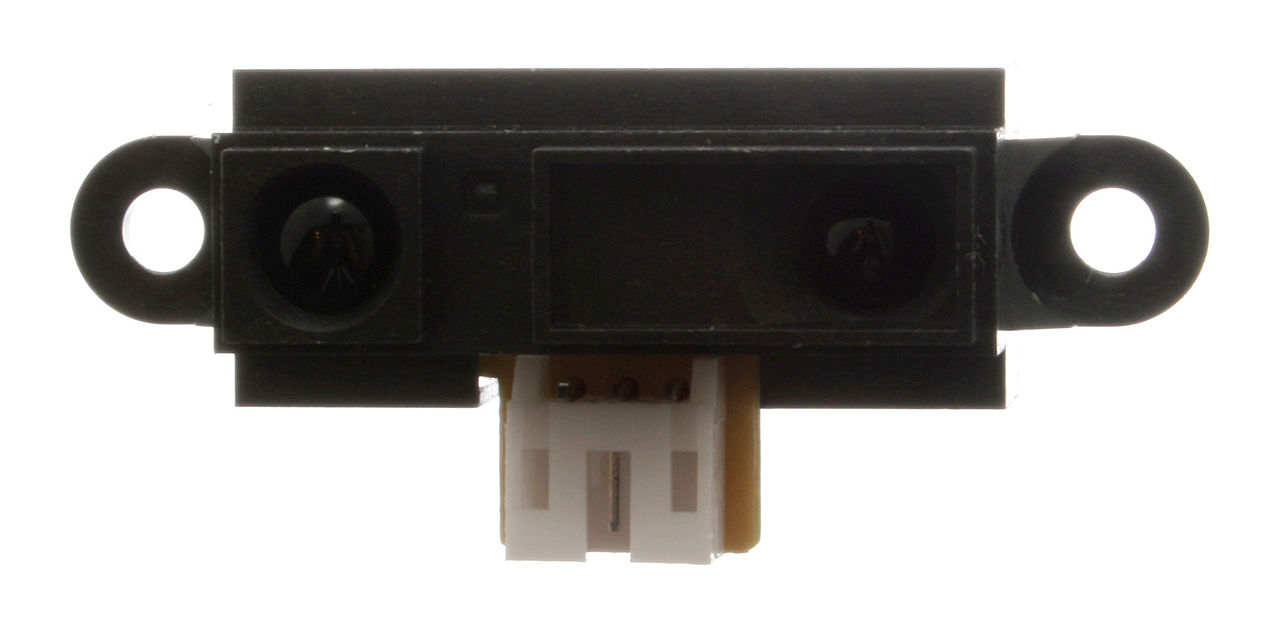
\includegraphics[scale=0.5]{images/proximity_sensor.jpg}
				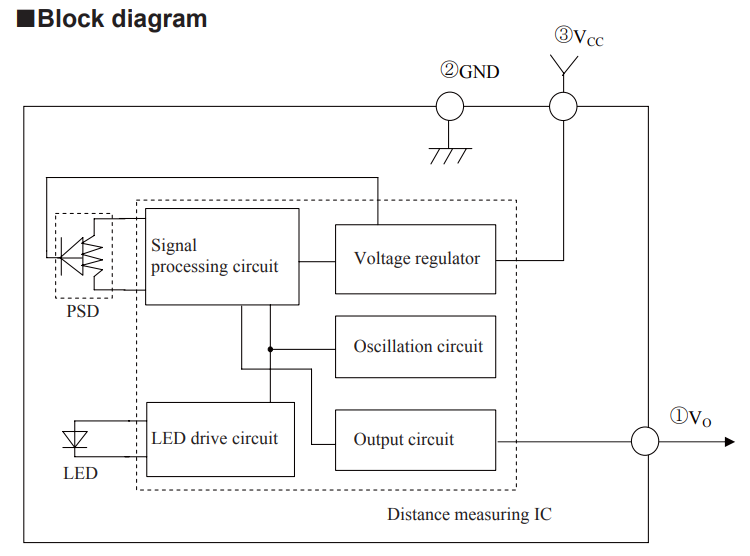
\includegraphics[scale=0.19]{images/sharp_ranger_circuit.png} \vspccc

				Identify the following measurement stages 
				\begin{itemize}
				\item Sensor: \hspcu
				\item Transducer: \hspcu
				\item Signal Conditioning: \hspcu
				\item Output: \hspcu
				\end{itemize}

				Name at least one for each of the following categories 

				\begin{itemize}
				\item Measured Variable: \hspcu \vspc 
				\item Independent Variable(s): \hspcu \vspc
				\item Dependent Variable(s): \hspcu, \hspcu \vspc 
				\item Controlled Variable(s): \hspcu, \hspcu \vspc 
				\item Extraneous Variable(s):\hspcu \vspc
				\end{itemize}

				\end{multicols}	

				{\tiny Image, More Info: \href{https://en.wikipedia.org/wiki/Proximity_sensor}{Wikipedia} }\hspace{40mm} {\tiny Image, More Info: \href{https://en.wikipedia.org/wiki/Position_sensitive_device}{Wikipedia} }

			\end{frame}

			% section II subsection V frame II
			\begin{frame}
				\frametitle{\sectionIIsubsectionVtitle}
				\tiny

				Indiviual Activity: Complete the activity and submit your work on ilearn {\it as an individual}.	

				\begin{multicols}{2}

				\textbf{Example 2: Thermocouple with DMM} \vspc
				\includegraphics[scale=0.35]{images/thermocouple_atd.png} \vspc

				Identify the following measurement stages 
				\begin{itemize}
				\item Sensor: \hspcu
				\item Transducer: \hspcu
				\item Signal Conditioning: \hspcu
				\item Output: \hspcu
				\end{itemize}


				Name at least one for each category 

				\begin{itemize}
				\item Measured Variable: \hspcu \vspc 
				\item Independent Variable(s): \hspcu, \hspcu \vspc
				\item Dependent Variable(s): \hspcu, \hspcu \vspc 
				\item Controlled Variable(s): \hspcu \vspc 
				\item Extraneous Variable(s):\hspcu \vspc
				\end{itemize}

				\end{multicols}	

				{\tiny Image, More Info: \href{https://en.wikipedia.org/wiki/Thermocouple}{Wikipedia} }\hspace{40mm} 

			\end{frame}


	% Section III
	\section{\sectionIIItitle}\label{sectionIII}

		% section III Outline
		\begin{frame}
			\large \textbf{Topic 3 - \sectionIIItitle} \vspace{3mm}\\

			\begin{itemize}
				\item \hyperlink{sectionIIIsubsectionI}{\sectionIIIsubsectionItitle} \vspc %  section III subsection I
				\item \hyperlink{sectionIIIsubsectionII}{\sectionIIIsubsectionIItitle} \vspc % section III subsection II
				\item \hyperlink{sectionIIIsubsectionIII}{\sectionIIIsubsectionIIItitle} \vspc % section III subsection III
				\item \hyperlink{sectionIIIsubsectionIV}{\sectionIIIsubsectionIVtitle} \vspc % section III subsection IV
			\end{itemize}
		\end{frame}

		% section III subsection I
		\subsection{\sectionIIIsubsectionItitle}\label{sectionIIIsubsectionI}

			\begin{frame}
				\frametitle{\sectionIIIsubsectionItitle}

				{\BL Parameter Design Plan}: Determine the test objective and identify the process variables and
				parameters and a means for their control. \vspc
				\underline{Ask}: \begin{itemize}
				\item What question am I trying to answer?
				\item What needs to be measured?
				\item What variables and parameters will affect my results?
				\end{itemize} 

				{\tiny Text: Theory and Design of Mech. Meas.}
			\end{frame}

		% section III subsection II
		\subsection{\sectionIIIsubsectionIItitle}\label{sectionIIIsubsectionII}	

			\begin{frame}
				\frametitle{\sectionIIIsubsectionIItitle}

				{\PR System and Tolerance Design Plan}: Select a measurement technique, equipment, and
				test procedure based on some preconceived tolerance limits for error. \vspc
				\underline{Ask}:
				\begin{itemize}
				\item In what ways can I do the measurement?
				\item How good do the results need to be to answer my
				question? 
				\end{itemize} 

				{\tiny Text: Theory and Design of Mech. Meas.}
			\end{frame}

		% section III subsection III
		\subsection{\sectionIIIsubsectionIItitle}\label{sectionIIIsubsectionIII}

			\begin{frame}
				\frametitle{\sectionIIIsubsectionIIItitle}

				{\GR Data Reduction Design Plan}: Plan how to analyze, present, and use the anticipated data.\vspc
				\underline{Ask}:
				\begin{itemize}
				\item How will I interpret the resulting data?
				\item How will I use the data to answer my question?
				\item How good is my answer? 
				\item Does my answer make sense?
				\end{itemize} 

				{\tiny Text: Theory and Design of Mech. Meas.}
			\end{frame}

		% section III subsection IV
		\subsection{\sectionIIIsubsectionIVtitle}\label{sectionIIIsubsectionIV}	

			\begin{frame}
				\frametitle{\sectionIIIsubsectionIVtitle}

				\begin{itemize}
					\item {\BL Randomized} Tests \vspccc% Section 1
					\item {\GR Repetition} and {\PR Replication}. \vspccc% Section 1
					\item {\BR Concomitant} Methods \vspccc
				\end{itemize}

			\end{frame}
	
		% section III subsection V
		\subsection{\sectionIIIsubsectionVtitle}\label{sectionIIIsubsectionV}

			\begin{frame}
				\frametitle{\sectionIIIsubsectionVtitle}
				\tiny

				Group Activity: Find a group of 2-3 students. Complete the activity and submit your work on ilearn {\it as an indiviual}. You may submit the same or similar answers as your group members.	

				\begin{multicols}{2}
					\textbf{Experimental Test Plan: Fuel/Energy Economy} \\
					%\includegraphics[scale=0.35]{thermocouple_atd.png} \vspc

					\begin{enumerate}
						\item Develop an experimental test plan for determining the milage cost of your vehicle (choose any vehicle) in dollars per mile. Write a short desciption of the system. (paragraph or bulleted list)
						\vspace{5mm}
						\item Identify the following variables for your plan.

						\begin{multicols}{2}
							\begin{itemize}\tiny
								\item Measured Variable: 
								\item Independent Variable(s): 
								\item Dependent Variable(s): 
								\item Controlled Variable(s): 
								\item Extraneous Variable(s):
							\end{itemize}
						\end{multicols}	

						\vspace{12mm}
						\item Do you expect the results of the study to represent the true milage of the vehicle? How could you validate (or check) the results?
						\item What could you do to improve the results of the proposed study?

					\end{enumerate}
				\end{multicols}	

				{\tiny Image, More Info: \href{https://en.wikipedia.org/wiki/Thermocouple}{Wikipedia} }\hspace{40mm} 

			\end{frame}			


	% Section IV
	\section{\sectionIVtitle}\label{sectionIV}



\end{document}





